\section{Поиск лёгких аксион-подобных частиц}

Частицы ALP имеют предсказанную распадную ширину
$\Gamma_{a} = g^2_{a\gamma\gamma} m_a^3 / 64 \pi$, что
в диапазоне масс в десятки и сотни ГэВ и значениях константы
смешивания $g_{a\gamma\gamma} \simeq10^{-5}$ соответствует
средней длине пробега в несколько метров. Таким образом,
условия NA64 могут позволять проверку существования гипотетических
частиц в диапазоне масс $10~\text{ГэВ} \lesssim m_a \lesssim 100~\text{ГэВ}$
и $10^{-4}\lesssim g_{a\gamma\gamma} \lesssim10^{-1}$, при условии
подавления сопутствующего фона.
Для этого нужно анализировать события, ожидая что
$a$ появится ECAL и в дальнейшем либо пройдёт первый модуль HCAL без
взаимодействия (невидимый канал), и либо распадётся в модулях HCAL ниже
по пучку (видимый канал).

Оба канала реакции рождения ALP детектируются по
отсутствию заметной доли энергии в ECAL, т.е. $E_{ECAL} < E_0$,
и отсутствию сигнала в вето, $E_{VETO} \approx 0$. Отличие состоит
в том, что для видимого канала необходимо ожидать энерговыделения
в HCAL2,3,4 -- $\sum\limits_{i = 3,4} E_{HCAL,i} > 0$.

Практически, условия ограничивающие энерговыделение должны определяться более
строго, из консервативных оценок неопределённостей возникающих
в реконструкции сигналов, а так же с учётом источников фона.
Например, для оценки вероятности MIP-частицы пройти тонкий
сцинтиллятор из \acrshort{pmma} толщиной $20~\text{мм}$ (VETO) с энерговыделением
менее половины $E_{MIP}/2 = 5{,}4/2~\text{МэВ}$, с точки зрения ионизационных
потерь составляет менее $10^{-40}$~(левая хвостовая вероятность распределения
Ландау). Таким образом (требуя $E_{VETO} < E_{MIP}/2$) можно
эффективно идентифицировать и исключить заряженные частицы. На
практике необходимо учитывать флуктуации светосбора и фотостатстики,
которые способны снизить эффективность такого метода непосредственного
детектирования заряженных частиц.
Такой учёт требует эмпирического уточнения оценок на основе данных.

Помимо статистических эффектов, в сигнальной параметрической области
видимого канала присутствуют дополнительные фоновые
процессы. Статистически-обоснованный
тест для гипотезы превышения сигнала над фоном сформулирован в методе
CLs~\cite{read-cls}, для которого необходимо получить количественные
оценки фоновых процессов.

%В общих чертах, метод включает 1) получение грубых оценок на основе
%общефизических соображений, 2) получение более точных оценок на
%основе \acrshort{mc}-моделей, 3) использование эталонных процессов
%для уточнения (валидации) или перенормировки оценок полученных
%при помощи моделирования.

\subsection{Идентификация адронного ливня}

Фон для сигнатуры $E_{HCAL1} < E_{\text{MIP}}/2$ (видимый канал)
создают в основном реакции рождения нейтральных адронов (каонов в и нейтронов)
на ядре в процессах $e^{-}Z\rightarrow n(K^0) + m\cdot\pi^0 + X$~---
т.н. \emph{leading neutrons} (англ.)~\cite{leading-neutron-hera}.
Эти частицы вызывают адронный ливень в HCAL, имеющий
в среднем более широкое пространственное распределение энергии,
чем ожидаемый в гипотетическом
распаде $a\rightarrow\gamma\gamma$ электромагнитный ливень.
Таким образом, проблема идентификация частицы
может быть решена за счёт гранулярности HCAL.
Таким образом, эффективным критерием, слабо зависящим от энергии
инициирующей частицы является ограничение на
значение относительной доли энерговыделение в периферийных ячейках --
$R = (E_{HCAL} - E_{HCAL,C})/E_{HCAL} < R_{th}$.
Чтобы приблизительно оценить оптимальный порог $R_{th}$
и статистическую мощность такого критерия можно использовать оценки
на основе \acrshort{mc}-моделирования.

На рисунке \ref{fig:var-ptype-ratios} приведены графики относительного
энерговыделения в периферийных ячейках $R$ для различных типов
инициирующей частицы. В моделировании использовался параллельный
радиально-симметричный пучок частиц с нормальным координатным
распределением со среднеквадратичным
отклонением~$\sigma_{x,y}=50~\text{мм}$.
\begin{figure}[ht]
    \centering
    \resizebox{!}{.35\textwidth}{% GNUPLOT: LaTeX picture with Postscript
\begingroup
  \makeatletter
  \providecommand\color[2][]{%
    \GenericError{(gnuplot) \space\space\space\@spaces}{%
      Package color not loaded in conjunction with
      terminal option `colourtext'%
    }{See the gnuplot documentation for explanation.%
    }{Either use 'blacktext' in gnuplot or load the package
      color.sty in LaTeX.}%
    \renewcommand\color[2][]{}%
  }%
  \providecommand\includegraphics[2][]{%
    \GenericError{(gnuplot) \space\space\space\@spaces}{%
      Package graphicx or graphics not loaded%
    }{See the gnuplot documentation for explanation.%
    }{The gnuplot epslatex terminal needs graphicx.sty or graphics.sty.}%
    \renewcommand\includegraphics[2][]{}%
  }%
  \providecommand\rotatebox[2]{#2}%
  \@ifundefined{ifGPcolor}{%
    \newif\ifGPcolor
    \GPcolorfalse
  }{}%
  \@ifundefined{ifGPblacktext}{%
    \newif\ifGPblacktext
    \GPblacktexttrue
  }{}%
  % define a \g@addto@macro without @ in the name:
  \let\gplgaddtomacro\g@addto@macro
  % define empty templates for all commands taking text:
  \gdef\gplbacktext{}%
  \gdef\gplfronttext{}%
  \makeatother
  \ifGPblacktext
    % no textcolor at all
    \def\colorrgb#1{}%
    \def\colorgray#1{}%
  \else
    % gray or color?
    \ifGPcolor
      \def\colorrgb#1{\color[rgb]{#1}}%
      \def\colorgray#1{\color[gray]{#1}}%
      \expandafter\def\csname LTw\endcsname{\color{white}}%
      \expandafter\def\csname LTb\endcsname{\color{black}}%
      \expandafter\def\csname LTa\endcsname{\color{black}}%
      \expandafter\def\csname LT0\endcsname{\color[rgb]{1,0,0}}%
      \expandafter\def\csname LT1\endcsname{\color[rgb]{0,1,0}}%
      \expandafter\def\csname LT2\endcsname{\color[rgb]{0,0,1}}%
      \expandafter\def\csname LT3\endcsname{\color[rgb]{1,0,1}}%
      \expandafter\def\csname LT4\endcsname{\color[rgb]{0,1,1}}%
      \expandafter\def\csname LT5\endcsname{\color[rgb]{1,1,0}}%
      \expandafter\def\csname LT6\endcsname{\color[rgb]{0,0,0}}%
      \expandafter\def\csname LT7\endcsname{\color[rgb]{1,0.3,0}}%
      \expandafter\def\csname LT8\endcsname{\color[rgb]{0.5,0.5,0.5}}%
    \else
      % gray
      \def\colorrgb#1{\color{black}}%
      \def\colorgray#1{\color[gray]{#1}}%
      \expandafter\def\csname LTw\endcsname{\color{white}}%
      \expandafter\def\csname LTb\endcsname{\color{black}}%
      \expandafter\def\csname LTa\endcsname{\color{black}}%
      \expandafter\def\csname LT0\endcsname{\color{black}}%
      \expandafter\def\csname LT1\endcsname{\color{black}}%
      \expandafter\def\csname LT2\endcsname{\color{black}}%
      \expandafter\def\csname LT3\endcsname{\color{black}}%
      \expandafter\def\csname LT4\endcsname{\color{black}}%
      \expandafter\def\csname LT5\endcsname{\color{black}}%
      \expandafter\def\csname LT6\endcsname{\color{black}}%
      \expandafter\def\csname LT7\endcsname{\color{black}}%
      \expandafter\def\csname LT8\endcsname{\color{black}}%
    \fi
  \fi
    \setlength{\unitlength}{0.0500bp}%
    \ifx\gptboxheight\undefined%
      \newlength{\gptboxheight}%
      \newlength{\gptboxwidth}%
      \newsavebox{\gptboxtext}%
    \fi%
    \setlength{\fboxrule}{0.5pt}%
    \setlength{\fboxsep}{1pt}%
    \definecolor{tbcol}{rgb}{1,1,1}%
\begin{picture}(5760.00,4320.00)%
    \gplgaddtomacro\gplbacktext{%
      \csname LTb\endcsname%%
      \put(946,4099){\makebox(0,0)[r]{\strut{}$1$}}%
      \put(946,704){\makebox(0,0)[r]{\strut{}$10^{-5}$}}%
      \put(946,1383){\makebox(0,0)[r]{\strut{}$10^{-4}$}}%
      \put(946,2062){\makebox(0,0)[r]{\strut{}$10^{-3}$}}%
      \put(946,2741){\makebox(0,0)[r]{\strut{}$10^{-2}$}}%
      \put(946,3420){\makebox(0,0)[r]{\strut{}$10^{-1}$}}%
      \put(1078,484){\makebox(0,0){\strut{}$0.01$}}%
      \put(3220,484){\makebox(0,0){\strut{}$0.1$}}%
    }%
    \gplgaddtomacro\gplfronttext{%
      \csname LTb\endcsname%%
      \put(4376,3926){\makebox(0,0)[r]{\strut{}$100~\text{ГэВ}$}}%
      \csname LTb\endcsname%%
      \put(4376,3706){\makebox(0,0)[r]{\strut{}$50~\text{ГэВ}$}}%
      \csname LTb\endcsname%%
      \put(4376,3486){\makebox(0,0)[r]{\strut{}$20~\text{ГэВ}$}}%
      \put(209,2401){\rotatebox{-270.00}{\makebox(0,0){\strut{}$p(E)$}}}%
      \put(3220,154){\makebox(0,0){\strut{}$R_{\gamma}$}}%
    }%
    \gplbacktext
    \put(0,0){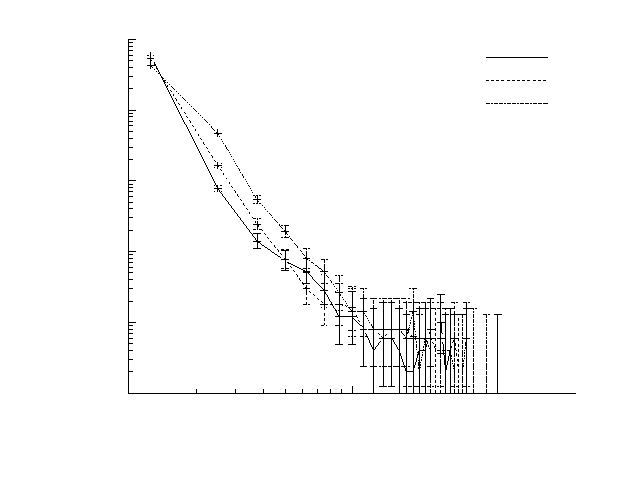
\includegraphics[width={288.00bp},height={216.00bp}]{images/r-simulations/different-types/lowerstatslowerstats-5e44f123_gamma.eps}}%
    \gplfronttext
  \end{picture}%
\endgroup
}
    \resizebox{!}{.35\textwidth}{% GNUPLOT: LaTeX picture with Postscript
\begingroup
  \makeatletter
  \providecommand\color[2][]{%
    \GenericError{(gnuplot) \space\space\space\@spaces}{%
      Package color not loaded in conjunction with
      terminal option `colourtext'%
    }{See the gnuplot documentation for explanation.%
    }{Either use 'blacktext' in gnuplot or load the package
      color.sty in LaTeX.}%
    \renewcommand\color[2][]{}%
  }%
  \providecommand\includegraphics[2][]{%
    \GenericError{(gnuplot) \space\space\space\@spaces}{%
      Package graphicx or graphics not loaded%
    }{See the gnuplot documentation for explanation.%
    }{The gnuplot epslatex terminal needs graphicx.sty or graphics.sty.}%
    \renewcommand\includegraphics[2][]{}%
  }%
  \providecommand\rotatebox[2]{#2}%
  \@ifundefined{ifGPcolor}{%
    \newif\ifGPcolor
    \GPcolorfalse
  }{}%
  \@ifundefined{ifGPblacktext}{%
    \newif\ifGPblacktext
    \GPblacktexttrue
  }{}%
  % define a \g@addto@macro without @ in the name:
  \let\gplgaddtomacro\g@addto@macro
  % define empty templates for all commands taking text:
  \gdef\gplbacktext{}%
  \gdef\gplfronttext{}%
  \makeatother
  \ifGPblacktext
    % no textcolor at all
    \def\colorrgb#1{}%
    \def\colorgray#1{}%
  \else
    % gray or color?
    \ifGPcolor
      \def\colorrgb#1{\color[rgb]{#1}}%
      \def\colorgray#1{\color[gray]{#1}}%
      \expandafter\def\csname LTw\endcsname{\color{white}}%
      \expandafter\def\csname LTb\endcsname{\color{black}}%
      \expandafter\def\csname LTa\endcsname{\color{black}}%
      \expandafter\def\csname LT0\endcsname{\color[rgb]{1,0,0}}%
      \expandafter\def\csname LT1\endcsname{\color[rgb]{0,1,0}}%
      \expandafter\def\csname LT2\endcsname{\color[rgb]{0,0,1}}%
      \expandafter\def\csname LT3\endcsname{\color[rgb]{1,0,1}}%
      \expandafter\def\csname LT4\endcsname{\color[rgb]{0,1,1}}%
      \expandafter\def\csname LT5\endcsname{\color[rgb]{1,1,0}}%
      \expandafter\def\csname LT6\endcsname{\color[rgb]{0,0,0}}%
      \expandafter\def\csname LT7\endcsname{\color[rgb]{1,0.3,0}}%
      \expandafter\def\csname LT8\endcsname{\color[rgb]{0.5,0.5,0.5}}%
    \else
      % gray
      \def\colorrgb#1{\color{black}}%
      \def\colorgray#1{\color[gray]{#1}}%
      \expandafter\def\csname LTw\endcsname{\color{white}}%
      \expandafter\def\csname LTb\endcsname{\color{black}}%
      \expandafter\def\csname LTa\endcsname{\color{black}}%
      \expandafter\def\csname LT0\endcsname{\color{black}}%
      \expandafter\def\csname LT1\endcsname{\color{black}}%
      \expandafter\def\csname LT2\endcsname{\color{black}}%
      \expandafter\def\csname LT3\endcsname{\color{black}}%
      \expandafter\def\csname LT4\endcsname{\color{black}}%
      \expandafter\def\csname LT5\endcsname{\color{black}}%
      \expandafter\def\csname LT6\endcsname{\color{black}}%
      \expandafter\def\csname LT7\endcsname{\color{black}}%
      \expandafter\def\csname LT8\endcsname{\color{black}}%
    \fi
  \fi
    \setlength{\unitlength}{0.0500bp}%
    \ifx\gptboxheight\undefined%
      \newlength{\gptboxheight}%
      \newlength{\gptboxwidth}%
      \newsavebox{\gptboxtext}%
    \fi%
    \setlength{\fboxrule}{0.5pt}%
    \setlength{\fboxsep}{1pt}%
    \definecolor{tbcol}{rgb}{1,1,1}%
\begin{picture}(5760.00,4320.00)%
    \gplgaddtomacro\gplbacktext{%
      \csname LTb\endcsname%%
      \put(946,4099){\makebox(0,0)[r]{\strut{}$1$}}%
      \put(946,704){\makebox(0,0)[r]{\strut{}$10^{-5}$}}%
      \put(946,1383){\makebox(0,0)[r]{\strut{}$10^{-4}$}}%
      \put(946,2062){\makebox(0,0)[r]{\strut{}$10^{-3}$}}%
      \put(946,2741){\makebox(0,0)[r]{\strut{}$10^{-2}$}}%
      \put(946,3420){\makebox(0,0)[r]{\strut{}$10^{-1}$}}%
      \put(1078,484){\makebox(0,0){\strut{}$0.01$}}%
      \put(3220,484){\makebox(0,0){\strut{}$0.1$}}%
    }%
    \gplgaddtomacro\gplfronttext{%
      \csname LTb\endcsname%%
      \put(4376,3926){\makebox(0,0)[r]{\strut{}$100~\text{ГэВ}$}}%
      \csname LTb\endcsname%%
      \put(4376,3706){\makebox(0,0)[r]{\strut{}$50~\text{ГэВ}$}}%
      \csname LTb\endcsname%%
      \put(4376,3486){\makebox(0,0)[r]{\strut{}$20~\text{ГэВ}$}}%
      \put(209,2401){\rotatebox{-270.00}{\makebox(0,0){\strut{}$p(E)$}}}%
      \put(3220,154){\makebox(0,0){\strut{}$R_{n}$}}%
    }%
    \gplbacktext
    \put(0,0){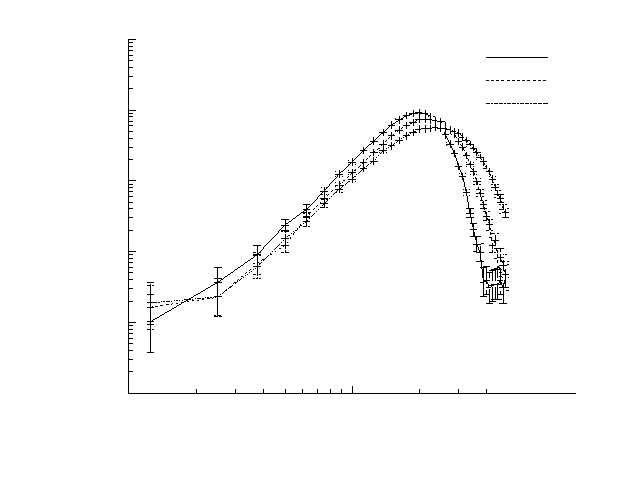
\includegraphics[width={288.00bp},height={216.00bp}]{images/r-simulations/different-types/lowerstatslowerstats-5e44f123_neutron.eps}}%
    \gplfronttext
  \end{picture}%
\endgroup
}
    \resizebox{!}{.35\textwidth}{% GNUPLOT: LaTeX picture with Postscript
\begingroup
  \makeatletter
  \providecommand\color[2][]{%
    \GenericError{(gnuplot) \space\space\space\@spaces}{%
      Package color not loaded in conjunction with
      terminal option `colourtext'%
    }{See the gnuplot documentation for explanation.%
    }{Either use 'blacktext' in gnuplot or load the package
      color.sty in LaTeX.}%
    \renewcommand\color[2][]{}%
  }%
  \providecommand\includegraphics[2][]{%
    \GenericError{(gnuplot) \space\space\space\@spaces}{%
      Package graphicx or graphics not loaded%
    }{See the gnuplot documentation for explanation.%
    }{The gnuplot epslatex terminal needs graphicx.sty or graphics.sty.}%
    \renewcommand\includegraphics[2][]{}%
  }%
  \providecommand\rotatebox[2]{#2}%
  \@ifundefined{ifGPcolor}{%
    \newif\ifGPcolor
    \GPcolorfalse
  }{}%
  \@ifundefined{ifGPblacktext}{%
    \newif\ifGPblacktext
    \GPblacktexttrue
  }{}%
  % define a \g@addto@macro without @ in the name:
  \let\gplgaddtomacro\g@addto@macro
  % define empty templates for all commands taking text:
  \gdef\gplbacktext{}%
  \gdef\gplfronttext{}%
  \makeatother
  \ifGPblacktext
    % no textcolor at all
    \def\colorrgb#1{}%
    \def\colorgray#1{}%
  \else
    % gray or color?
    \ifGPcolor
      \def\colorrgb#1{\color[rgb]{#1}}%
      \def\colorgray#1{\color[gray]{#1}}%
      \expandafter\def\csname LTw\endcsname{\color{white}}%
      \expandafter\def\csname LTb\endcsname{\color{black}}%
      \expandafter\def\csname LTa\endcsname{\color{black}}%
      \expandafter\def\csname LT0\endcsname{\color[rgb]{1,0,0}}%
      \expandafter\def\csname LT1\endcsname{\color[rgb]{0,1,0}}%
      \expandafter\def\csname LT2\endcsname{\color[rgb]{0,0,1}}%
      \expandafter\def\csname LT3\endcsname{\color[rgb]{1,0,1}}%
      \expandafter\def\csname LT4\endcsname{\color[rgb]{0,1,1}}%
      \expandafter\def\csname LT5\endcsname{\color[rgb]{1,1,0}}%
      \expandafter\def\csname LT6\endcsname{\color[rgb]{0,0,0}}%
      \expandafter\def\csname LT7\endcsname{\color[rgb]{1,0.3,0}}%
      \expandafter\def\csname LT8\endcsname{\color[rgb]{0.5,0.5,0.5}}%
    \else
      % gray
      \def\colorrgb#1{\color{black}}%
      \def\colorgray#1{\color[gray]{#1}}%
      \expandafter\def\csname LTw\endcsname{\color{white}}%
      \expandafter\def\csname LTb\endcsname{\color{black}}%
      \expandafter\def\csname LTa\endcsname{\color{black}}%
      \expandafter\def\csname LT0\endcsname{\color{black}}%
      \expandafter\def\csname LT1\endcsname{\color{black}}%
      \expandafter\def\csname LT2\endcsname{\color{black}}%
      \expandafter\def\csname LT3\endcsname{\color{black}}%
      \expandafter\def\csname LT4\endcsname{\color{black}}%
      \expandafter\def\csname LT5\endcsname{\color{black}}%
      \expandafter\def\csname LT6\endcsname{\color{black}}%
      \expandafter\def\csname LT7\endcsname{\color{black}}%
      \expandafter\def\csname LT8\endcsname{\color{black}}%
    \fi
  \fi
    \setlength{\unitlength}{0.0500bp}%
    \ifx\gptboxheight\undefined%
      \newlength{\gptboxheight}%
      \newlength{\gptboxwidth}%
      \newsavebox{\gptboxtext}%
    \fi%
    \setlength{\fboxrule}{0.5pt}%
    \setlength{\fboxsep}{1pt}%
    \definecolor{tbcol}{rgb}{1,1,1}%
\begin{picture}(5760.00,4320.00)%
    \gplgaddtomacro\gplbacktext{%
      \csname LTb\endcsname%%
      \put(946,4099){\makebox(0,0)[r]{\strut{}$1$}}%
      \put(946,704){\makebox(0,0)[r]{\strut{}$10^{-5}$}}%
      \put(946,1383){\makebox(0,0)[r]{\strut{}$10^{-4}$}}%
      \put(946,2062){\makebox(0,0)[r]{\strut{}$10^{-3}$}}%
      \put(946,2741){\makebox(0,0)[r]{\strut{}$10^{-2}$}}%
      \put(946,3420){\makebox(0,0)[r]{\strut{}$10^{-1}$}}%
      \put(1078,484){\makebox(0,0){\strut{}$0.01$}}%
      \put(3220,484){\makebox(0,0){\strut{}$0.1$}}%
    }%
    \gplgaddtomacro\gplfronttext{%
      \csname LTb\endcsname%%
      \put(4376,3926){\makebox(0,0)[r]{\strut{}$100~\text{ГэВ}$}}%
      \csname LTb\endcsname%%
      \put(4376,3706){\makebox(0,0)[r]{\strut{}$50~\text{ГэВ}$}}%
      \csname LTb\endcsname%%
      \put(4376,3486){\makebox(0,0)[r]{\strut{}$20~\text{ГэВ}$}}%
      \put(209,2401){\rotatebox{-270.00}{\makebox(0,0){\strut{}$p(E)$}}}%
      \put(3220,154){\makebox(0,0){\strut{}$R_{\pi^{-}}$}}%
    }%
    \gplbacktext
    \put(0,0){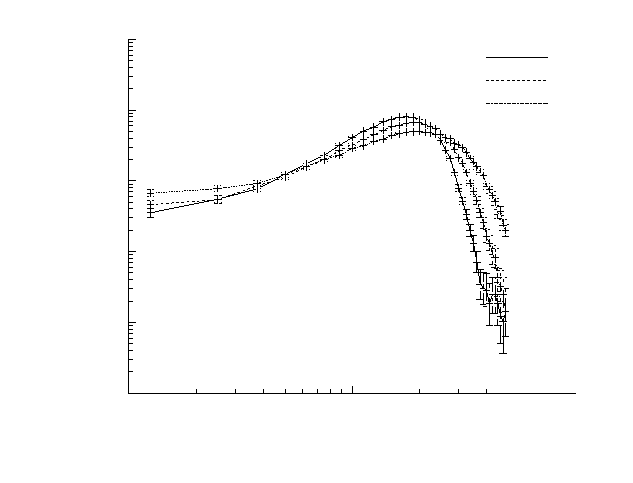
\includegraphics[width={288.00bp},height={216.00bp}]{images/r-simulations/different-types/lowerstatslowerstats-5e44f123_pi-.eps}}%
    \gplfronttext
  \end{picture}%
\endgroup
}
    \resizebox{!}{.35\textwidth}{% GNUPLOT: LaTeX picture with Postscript
\begingroup
  \makeatletter
  \providecommand\color[2][]{%
    \GenericError{(gnuplot) \space\space\space\@spaces}{%
      Package color not loaded in conjunction with
      terminal option `colourtext'%
    }{See the gnuplot documentation for explanation.%
    }{Either use 'blacktext' in gnuplot or load the package
      color.sty in LaTeX.}%
    \renewcommand\color[2][]{}%
  }%
  \providecommand\includegraphics[2][]{%
    \GenericError{(gnuplot) \space\space\space\@spaces}{%
      Package graphicx or graphics not loaded%
    }{See the gnuplot documentation for explanation.%
    }{The gnuplot epslatex terminal needs graphicx.sty or graphics.sty.}%
    \renewcommand\includegraphics[2][]{}%
  }%
  \providecommand\rotatebox[2]{#2}%
  \@ifundefined{ifGPcolor}{%
    \newif\ifGPcolor
    \GPcolorfalse
  }{}%
  \@ifundefined{ifGPblacktext}{%
    \newif\ifGPblacktext
    \GPblacktexttrue
  }{}%
  % define a \g@addto@macro without @ in the name:
  \let\gplgaddtomacro\g@addto@macro
  % define empty templates for all commands taking text:
  \gdef\gplbacktext{}%
  \gdef\gplfronttext{}%
  \makeatother
  \ifGPblacktext
    % no textcolor at all
    \def\colorrgb#1{}%
    \def\colorgray#1{}%
  \else
    % gray or color?
    \ifGPcolor
      \def\colorrgb#1{\color[rgb]{#1}}%
      \def\colorgray#1{\color[gray]{#1}}%
      \expandafter\def\csname LTw\endcsname{\color{white}}%
      \expandafter\def\csname LTb\endcsname{\color{black}}%
      \expandafter\def\csname LTa\endcsname{\color{black}}%
      \expandafter\def\csname LT0\endcsname{\color[rgb]{1,0,0}}%
      \expandafter\def\csname LT1\endcsname{\color[rgb]{0,1,0}}%
      \expandafter\def\csname LT2\endcsname{\color[rgb]{0,0,1}}%
      \expandafter\def\csname LT3\endcsname{\color[rgb]{1,0,1}}%
      \expandafter\def\csname LT4\endcsname{\color[rgb]{0,1,1}}%
      \expandafter\def\csname LT5\endcsname{\color[rgb]{1,1,0}}%
      \expandafter\def\csname LT6\endcsname{\color[rgb]{0,0,0}}%
      \expandafter\def\csname LT7\endcsname{\color[rgb]{1,0.3,0}}%
      \expandafter\def\csname LT8\endcsname{\color[rgb]{0.5,0.5,0.5}}%
    \else
      % gray
      \def\colorrgb#1{\color{black}}%
      \def\colorgray#1{\color[gray]{#1}}%
      \expandafter\def\csname LTw\endcsname{\color{white}}%
      \expandafter\def\csname LTb\endcsname{\color{black}}%
      \expandafter\def\csname LTa\endcsname{\color{black}}%
      \expandafter\def\csname LT0\endcsname{\color{black}}%
      \expandafter\def\csname LT1\endcsname{\color{black}}%
      \expandafter\def\csname LT2\endcsname{\color{black}}%
      \expandafter\def\csname LT3\endcsname{\color{black}}%
      \expandafter\def\csname LT4\endcsname{\color{black}}%
      \expandafter\def\csname LT5\endcsname{\color{black}}%
      \expandafter\def\csname LT6\endcsname{\color{black}}%
      \expandafter\def\csname LT7\endcsname{\color{black}}%
      \expandafter\def\csname LT8\endcsname{\color{black}}%
    \fi
  \fi
    \setlength{\unitlength}{0.0500bp}%
    \ifx\gptboxheight\undefined%
      \newlength{\gptboxheight}%
      \newlength{\gptboxwidth}%
      \newsavebox{\gptboxtext}%
    \fi%
    \setlength{\fboxrule}{0.5pt}%
    \setlength{\fboxsep}{1pt}%
    \definecolor{tbcol}{rgb}{1,1,1}%
\begin{picture}(5760.00,4320.00)%
    \gplgaddtomacro\gplbacktext{%
      \csname LTb\endcsname%%
      \put(946,4099){\makebox(0,0)[r]{\strut{}$1$}}%
      \put(946,704){\makebox(0,0)[r]{\strut{}$10^{-5}$}}%
      \put(946,1383){\makebox(0,0)[r]{\strut{}$10^{-4}$}}%
      \put(946,2062){\makebox(0,0)[r]{\strut{}$10^{-3}$}}%
      \put(946,2741){\makebox(0,0)[r]{\strut{}$10^{-2}$}}%
      \put(946,3420){\makebox(0,0)[r]{\strut{}$10^{-1}$}}%
      \put(1078,484){\makebox(0,0){\strut{}$0.01$}}%
      \put(3220,484){\makebox(0,0){\strut{}$0.1$}}%
    }%
    \gplgaddtomacro\gplfronttext{%
      \csname LTb\endcsname%%
      \put(4376,3926){\makebox(0,0)[r]{\strut{}$100~\text{ГэВ}$}}%
      \csname LTb\endcsname%%
      \put(4376,3706){\makebox(0,0)[r]{\strut{}$50~\text{ГэВ}$}}%
      \csname LTb\endcsname%%
      \put(4376,3486){\makebox(0,0)[r]{\strut{}$20~\text{ГэВ}$}}%
      \put(209,2401){\rotatebox{-270.00}{\makebox(0,0){\strut{}$p(E)$}}}%
      \put(3220,154){\makebox(0,0){\strut{}$R_{\bar{K_0}}$}}%
    }%
    \gplbacktext
    \put(0,0){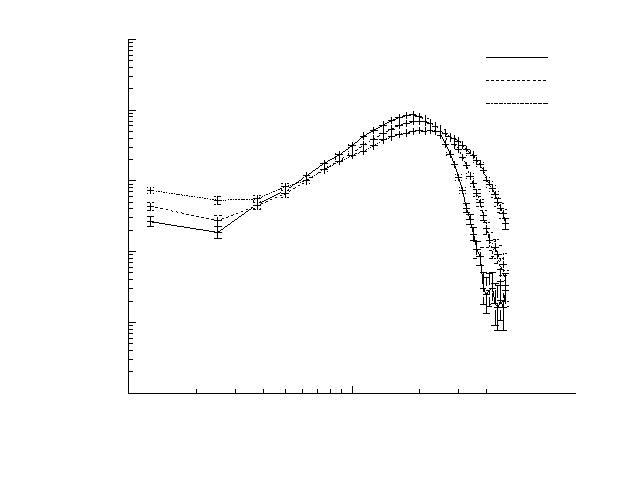
\includegraphics[width={288.00bp},height={216.00bp}]{images/r-simulations/different-types/lowerstatslowerstats-5e44f123_kaon0L.eps}}%
    \gplfronttext
  \end{picture}%
\endgroup
}
    \caption{Вероятности относительной доли энерговыделения $R$  % в HCAL2,3
    для различных энергий и типов инициирующей частицы согласно
    моделированию}
    \label{fig:var-ptype-ratios}
\end{figure}
Из рисунка следует, что вероятность периферийного энерговыделения
у $\gamma$-квантов (в области $R \lesssim 10^{-1}$) как
минимум на два порядка меньше таковой у нейтральных адронов при
достаточно малой относительной неопределённости.

% H_0 -- ливень адронный!
Пусть нулевая гипотеза $H_0$ состоит в том, что наблюдаемы ливень
является адронным. Тогда для критерия $R < R_{th}$ кривая
отражающая зависимость ошибок первого и второго рода приведена
На рисунке~\ref{fig:roc-curve-rfac}. На графике отмечена рабочая точка
$R_{th}^{(MC)} = 0{,}04$ при уровне статистической значимости
$\alpha=5\cdot10^{-3}$ (вероятность ошибочной идентификации
электромагнитного ливня как адронного) отвечает мощности
критерия $\beta_{R,0} = 0{,}994$
(вероятность корректной идентификации нейтрального адрона).
\begin{figure}[ht]
    \centering
    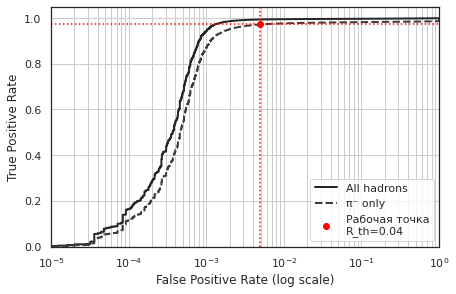
\includegraphics[width=0.65\linewidth]{images//r-simulations/roc-curve.png}
    \caption{ROC-кривая для критерия $R < R_{th}$ применяемого для разделения
    адронных и электромагнитных ливней в адронном калориметре}
    \label{fig:roc-curve-rfac}
\end{figure}
Для отрицательных пионов мощность несколько
ниже ($\beta_{R,\pi^{-}} = 0{,}972$) за счёт чуть б\'ольшей доли
компактных ливней вызванных, по-видимому, глубоко-неупругими реакциями
и реакциями перезарядки.

На практике, рабочая точка выбиралась исходя из оценок скорректированных
на основе отклика калориметра от реальных данных калибровочных пучков
$e^{-}$ и $\pi^{-}$. На рисунке \ref{fig:r-dist-realdata} в абсолютных
значениях показаны частоты событий соответствующих реальным и калибровочным
данным.
%Модельные распределения для обоих типов пучков показаны
%на рисунке~\ref{fig:r-distributions}, откуда видно, что $R$ для обоих
%типов событий слабо зависит от энергии.
%\begin{figure}[ht]
%    \centering
%    %\resizebox{!}{.4\textwidth}{% GNUPLOT: LaTeX picture with Postscript
\begingroup
  \makeatletter
  \providecommand\color[2][]{%
    \GenericError{(gnuplot) \space\space\space\@spaces}{%
      Package color not loaded in conjunction with
      terminal option `colourtext'%
    }{See the gnuplot documentation for explanation.%
    }{Either use 'blacktext' in gnuplot or load the package
      color.sty in LaTeX.}%
    \renewcommand\color[2][]{}%
  }%
  \providecommand\includegraphics[2][]{%
    \GenericError{(gnuplot) \space\space\space\@spaces}{%
      Package graphicx or graphics not loaded%
    }{See the gnuplot documentation for explanation.%
    }{The gnuplot epslatex terminal needs graphicx.sty or graphics.sty.}%
    \renewcommand\includegraphics[2][]{}%
  }%
  \providecommand\rotatebox[2]{#2}%
  \@ifundefined{ifGPcolor}{%
    \newif\ifGPcolor
    \GPcolorfalse
  }{}%
  \@ifundefined{ifGPblacktext}{%
    \newif\ifGPblacktext
    \GPblacktexttrue
  }{}%
  % define a \g@addto@macro without @ in the name:
  \let\gplgaddtomacro\g@addto@macro
  % define empty templates for all commands taking text:
  \gdef\gplbacktext{}%
  \gdef\gplfronttext{}%
  \makeatother
  \ifGPblacktext
    % no textcolor at all
    \def\colorrgb#1{}%
    \def\colorgray#1{}%
  \else
    % gray or color?
    \ifGPcolor
      \def\colorrgb#1{\color[rgb]{#1}}%
      \def\colorgray#1{\color[gray]{#1}}%
      \expandafter\def\csname LTw\endcsname{\color{white}}%
      \expandafter\def\csname LTb\endcsname{\color{black}}%
      \expandafter\def\csname LTa\endcsname{\color{black}}%
      \expandafter\def\csname LT0\endcsname{\color[rgb]{1,0,0}}%
      \expandafter\def\csname LT1\endcsname{\color[rgb]{0,1,0}}%
      \expandafter\def\csname LT2\endcsname{\color[rgb]{0,0,1}}%
      \expandafter\def\csname LT3\endcsname{\color[rgb]{1,0,1}}%
      \expandafter\def\csname LT4\endcsname{\color[rgb]{0,1,1}}%
      \expandafter\def\csname LT5\endcsname{\color[rgb]{1,1,0}}%
      \expandafter\def\csname LT6\endcsname{\color[rgb]{0,0,0}}%
      \expandafter\def\csname LT7\endcsname{\color[rgb]{1,0.3,0}}%
      \expandafter\def\csname LT8\endcsname{\color[rgb]{0.5,0.5,0.5}}%
    \else
      % gray
      \def\colorrgb#1{\color{black}}%
      \def\colorgray#1{\color[gray]{#1}}%
      \expandafter\def\csname LTw\endcsname{\color{white}}%
      \expandafter\def\csname LTb\endcsname{\color{black}}%
      \expandafter\def\csname LTa\endcsname{\color{black}}%
      \expandafter\def\csname LT0\endcsname{\color{black}}%
      \expandafter\def\csname LT1\endcsname{\color{black}}%
      \expandafter\def\csname LT2\endcsname{\color{black}}%
      \expandafter\def\csname LT3\endcsname{\color{black}}%
      \expandafter\def\csname LT4\endcsname{\color{black}}%
      \expandafter\def\csname LT5\endcsname{\color{black}}%
      \expandafter\def\csname LT6\endcsname{\color{black}}%
      \expandafter\def\csname LT7\endcsname{\color{black}}%
      \expandafter\def\csname LT8\endcsname{\color{black}}%
    \fi
  \fi
    \setlength{\unitlength}{0.0500bp}%
    \ifx\gptboxheight\undefined%
      \newlength{\gptboxheight}%
      \newlength{\gptboxwidth}%
      \newsavebox{\gptboxtext}%
    \fi%
    \setlength{\fboxrule}{0.5pt}%
    \setlength{\fboxsep}{1pt}%
    \definecolor{tbcol}{rgb}{1,1,1}%
\begin{picture}(5760.00,4320.00)%
    \gplgaddtomacro\gplbacktext{%
      \csname LTb\endcsname%%
      \put(946,4099){\makebox(0,0)[r]{\strut{}$1$}}%
      \put(946,704){\makebox(0,0)[r]{\strut{}$10^{-5}$}}%
      \put(946,1383){\makebox(0,0)[r]{\strut{}$10^{-4}$}}%
      \put(946,2062){\makebox(0,0)[r]{\strut{}$10^{-3}$}}%
      \put(946,2741){\makebox(0,0)[r]{\strut{}$10^{-2}$}}%
      \put(946,3420){\makebox(0,0)[r]{\strut{}$10^{-1}$}}%
      \put(1078,484){\makebox(0,0){\strut{}$0$}}%
      \put(1980,484){\makebox(0,0){\strut{}$0.1$}}%
      \put(2882,484){\makebox(0,0){\strut{}$0.2$}}%
      \put(3784,484){\makebox(0,0){\strut{}$0.3$}}%
      \put(4686,484){\makebox(0,0){\strut{}$0.4$}}%
    }%
    \gplgaddtomacro\gplfronttext{%
      \csname LTb\endcsname%%
      \put(4376,3926){\makebox(0,0)[r]{\strut{}$100~\text{ГэВ}$}}%
      \csname LTb\endcsname%%
      \put(4376,3706){\makebox(0,0)[r]{\strut{}$50~\text{ГэВ}$}}%
      \csname LTb\endcsname%%
      \put(4376,3486){\makebox(0,0)[r]{\strut{}$20~\text{ГэВ}$}}%
      \put(209,2401){\rotatebox{-270.00}{\makebox(0,0){\strut{}$p_{\pi^{-}}(E)$}}}%
      \put(3220,154){\makebox(0,0){\strut{}$R$}}%
    }%
    \gplbacktext
    \put(0,0){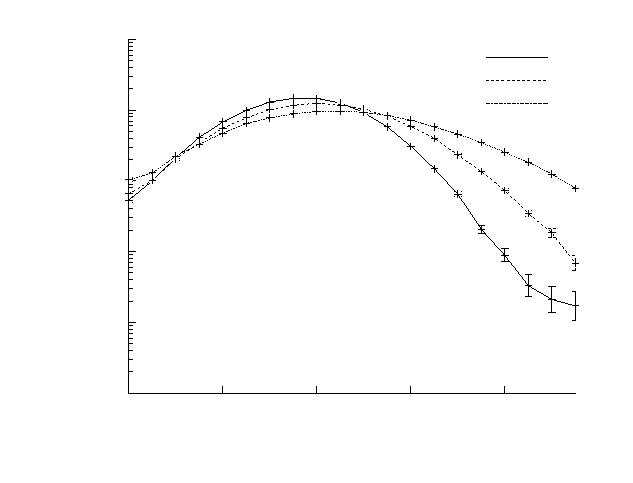
\includegraphics[width={288.00bp},height={216.00bp}]{images/r-simulations/pions-general-view.eps}}%
    \gplfronttext
  \end{picture}%
\endgroup
}
%    %\resizebox{!}{.65\textwidth}{% GNUPLOT: LaTeX picture with Postscript
\begingroup
  \makeatletter
  \providecommand\color[2][]{%
    \GenericError{(gnuplot) \space\space\space\@spaces}{%
      Package color not loaded in conjunction with
      terminal option `colourtext'%
    }{See the gnuplot documentation for explanation.%
    }{Either use 'blacktext' in gnuplot or load the package
      color.sty in LaTeX.}%
    \renewcommand\color[2][]{}%
  }%
  \providecommand\includegraphics[2][]{%
    \GenericError{(gnuplot) \space\space\space\@spaces}{%
      Package graphicx or graphics not loaded%
    }{See the gnuplot documentation for explanation.%
    }{The gnuplot epslatex terminal needs graphicx.sty or graphics.sty.}%
    \renewcommand\includegraphics[2][]{}%
  }%
  \providecommand\rotatebox[2]{#2}%
  \@ifundefined{ifGPcolor}{%
    \newif\ifGPcolor
    \GPcolorfalse
  }{}%
  \@ifundefined{ifGPblacktext}{%
    \newif\ifGPblacktext
    \GPblacktexttrue
  }{}%
  % define a \g@addto@macro without @ in the name:
  \let\gplgaddtomacro\g@addto@macro
  % define empty templates for all commands taking text:
  \gdef\gplbacktext{}%
  \gdef\gplfronttext{}%
  \makeatother
  \ifGPblacktext
    % no textcolor at all
    \def\colorrgb#1{}%
    \def\colorgray#1{}%
  \else
    % gray or color?
    \ifGPcolor
      \def\colorrgb#1{\color[rgb]{#1}}%
      \def\colorgray#1{\color[gray]{#1}}%
      \expandafter\def\csname LTw\endcsname{\color{white}}%
      \expandafter\def\csname LTb\endcsname{\color{black}}%
      \expandafter\def\csname LTa\endcsname{\color{black}}%
      \expandafter\def\csname LT0\endcsname{\color[rgb]{1,0,0}}%
      \expandafter\def\csname LT1\endcsname{\color[rgb]{0,1,0}}%
      \expandafter\def\csname LT2\endcsname{\color[rgb]{0,0,1}}%
      \expandafter\def\csname LT3\endcsname{\color[rgb]{1,0,1}}%
      \expandafter\def\csname LT4\endcsname{\color[rgb]{0,1,1}}%
      \expandafter\def\csname LT5\endcsname{\color[rgb]{1,1,0}}%
      \expandafter\def\csname LT6\endcsname{\color[rgb]{0,0,0}}%
      \expandafter\def\csname LT7\endcsname{\color[rgb]{1,0.3,0}}%
      \expandafter\def\csname LT8\endcsname{\color[rgb]{0.5,0.5,0.5}}%
    \else
      % gray
      \def\colorrgb#1{\color{black}}%
      \def\colorgray#1{\color[gray]{#1}}%
      \expandafter\def\csname LTw\endcsname{\color{white}}%
      \expandafter\def\csname LTb\endcsname{\color{black}}%
      \expandafter\def\csname LTa\endcsname{\color{black}}%
      \expandafter\def\csname LT0\endcsname{\color{black}}%
      \expandafter\def\csname LT1\endcsname{\color{black}}%
      \expandafter\def\csname LT2\endcsname{\color{black}}%
      \expandafter\def\csname LT3\endcsname{\color{black}}%
      \expandafter\def\csname LT4\endcsname{\color{black}}%
      \expandafter\def\csname LT5\endcsname{\color{black}}%
      \expandafter\def\csname LT6\endcsname{\color{black}}%
      \expandafter\def\csname LT7\endcsname{\color{black}}%
      \expandafter\def\csname LT8\endcsname{\color{black}}%
    \fi
  \fi
    \setlength{\unitlength}{0.0500bp}%
    \ifx\gptboxheight\undefined%
      \newlength{\gptboxheight}%
      \newlength{\gptboxwidth}%
      \newsavebox{\gptboxtext}%
    \fi%
    \setlength{\fboxrule}{0.5pt}%
    \setlength{\fboxsep}{1pt}%
    \definecolor{tbcol}{rgb}{1,1,1}%
\begin{picture}(5760.00,4320.00)%
    \gplgaddtomacro\gplbacktext{%
      \csname LTb\endcsname%%
      \put(946,4099){\makebox(0,0)[r]{\strut{}$1$}}%
      \put(946,704){\makebox(0,0)[r]{\strut{}$10^{-5}$}}%
      \put(946,1383){\makebox(0,0)[r]{\strut{}$10^{-4}$}}%
      \put(946,2062){\makebox(0,0)[r]{\strut{}$10^{-3}$}}%
      \put(946,2741){\makebox(0,0)[r]{\strut{}$10^{-2}$}}%
      \put(946,3420){\makebox(0,0)[r]{\strut{}$10^{-1}$}}%
      \put(1078,484){\makebox(0,0){\strut{}$0$}}%
      \put(1980,484){\makebox(0,0){\strut{}$0.1$}}%
      \put(2882,484){\makebox(0,0){\strut{}$0.2$}}%
      \put(3784,484){\makebox(0,0){\strut{}$0.3$}}%
      \put(4686,484){\makebox(0,0){\strut{}$0.4$}}%
    }%
    \gplgaddtomacro\gplfronttext{%
      \csname LTb\endcsname%%
      \put(4376,3926){\makebox(0,0)[r]{\strut{}$100~\text{ГэВ}$}}%
      \csname LTb\endcsname%%
      \put(4376,3706){\makebox(0,0)[r]{\strut{}$50~\text{ГэВ}$}}%
      \csname LTb\endcsname%%
      \put(4376,3486){\makebox(0,0)[r]{\strut{}$20~\text{ГэВ}$}}%
      \put(209,2401){\rotatebox{-270.00}{\makebox(0,0){\strut{}$p_{e^{-}}(E)$}}}%
      \put(3220,154){\makebox(0,0){\strut{}$R$}}%
    }%
    \gplbacktext
    \put(0,0){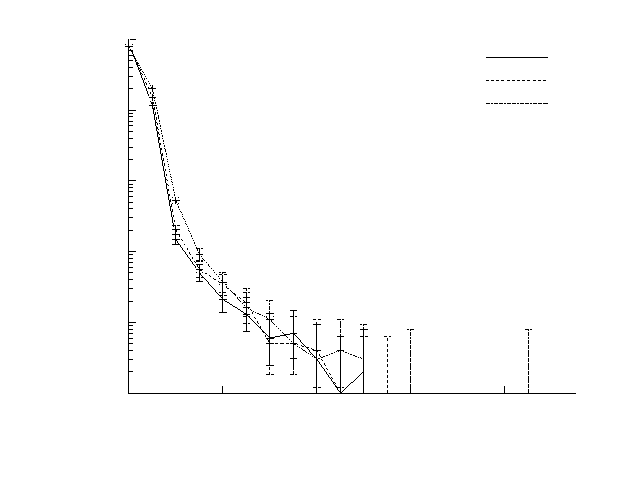
\includegraphics[width={288.00bp},height={216.00bp}]{images/r-simulations/electrons-general-view.eps}}%
    \gplfronttext
  \end{picture}%
\endgroup
}
%    \resizebox{!}{.33\textwidth}{% GNUPLOT: LaTeX picture with Postscript
\begingroup
  \makeatletter
  \providecommand\color[2][]{%
    \GenericError{(gnuplot) \space\space\space\@spaces}{%
      Package color not loaded in conjunction with
      terminal option `colourtext'%
    }{See the gnuplot documentation for explanation.%
    }{Either use 'blacktext' in gnuplot or load the package
      color.sty in LaTeX.}%
    \renewcommand\color[2][]{}%
  }%
  \providecommand\includegraphics[2][]{%
    \GenericError{(gnuplot) \space\space\space\@spaces}{%
      Package graphicx or graphics not loaded%
    }{See the gnuplot documentation for explanation.%
    }{The gnuplot epslatex terminal needs graphicx.sty or graphics.sty.}%
    \renewcommand\includegraphics[2][]{}%
  }%
  \providecommand\rotatebox[2]{#2}%
  \@ifundefined{ifGPcolor}{%
    \newif\ifGPcolor
    \GPcolorfalse
  }{}%
  \@ifundefined{ifGPblacktext}{%
    \newif\ifGPblacktext
    \GPblacktexttrue
  }{}%
  % define a \g@addto@macro without @ in the name:
  \let\gplgaddtomacro\g@addto@macro
  % define empty templates for all commands taking text:
  \gdef\gplbacktext{}%
  \gdef\gplfronttext{}%
  \makeatother
  \ifGPblacktext
    % no textcolor at all
    \def\colorrgb#1{}%
    \def\colorgray#1{}%
  \else
    % gray or color?
    \ifGPcolor
      \def\colorrgb#1{\color[rgb]{#1}}%
      \def\colorgray#1{\color[gray]{#1}}%
      \expandafter\def\csname LTw\endcsname{\color{white}}%
      \expandafter\def\csname LTb\endcsname{\color{black}}%
      \expandafter\def\csname LTa\endcsname{\color{black}}%
      \expandafter\def\csname LT0\endcsname{\color[rgb]{1,0,0}}%
      \expandafter\def\csname LT1\endcsname{\color[rgb]{0,1,0}}%
      \expandafter\def\csname LT2\endcsname{\color[rgb]{0,0,1}}%
      \expandafter\def\csname LT3\endcsname{\color[rgb]{1,0,1}}%
      \expandafter\def\csname LT4\endcsname{\color[rgb]{0,1,1}}%
      \expandafter\def\csname LT5\endcsname{\color[rgb]{1,1,0}}%
      \expandafter\def\csname LT6\endcsname{\color[rgb]{0,0,0}}%
      \expandafter\def\csname LT7\endcsname{\color[rgb]{1,0.3,0}}%
      \expandafter\def\csname LT8\endcsname{\color[rgb]{0.5,0.5,0.5}}%
    \else
      % gray
      \def\colorrgb#1{\color{black}}%
      \def\colorgray#1{\color[gray]{#1}}%
      \expandafter\def\csname LTw\endcsname{\color{white}}%
      \expandafter\def\csname LTb\endcsname{\color{black}}%
      \expandafter\def\csname LTa\endcsname{\color{black}}%
      \expandafter\def\csname LT0\endcsname{\color{black}}%
      \expandafter\def\csname LT1\endcsname{\color{black}}%
      \expandafter\def\csname LT2\endcsname{\color{black}}%
      \expandafter\def\csname LT3\endcsname{\color{black}}%
      \expandafter\def\csname LT4\endcsname{\color{black}}%
      \expandafter\def\csname LT5\endcsname{\color{black}}%
      \expandafter\def\csname LT6\endcsname{\color{black}}%
      \expandafter\def\csname LT7\endcsname{\color{black}}%
      \expandafter\def\csname LT8\endcsname{\color{black}}%
    \fi
  \fi
    \setlength{\unitlength}{0.0500bp}%
    \ifx\gptboxheight\undefined%
      \newlength{\gptboxheight}%
      \newlength{\gptboxwidth}%
      \newsavebox{\gptboxtext}%
    \fi%
    \setlength{\fboxrule}{0.5pt}%
    \setlength{\fboxsep}{1pt}%
    \definecolor{tbcol}{rgb}{1,1,1}%
\begin{picture}(5760.00,4320.00)%
    \gplgaddtomacro\gplbacktext{%
      \csname LTb\endcsname%%
      \put(946,4099){\makebox(0,0)[r]{\strut{}$1$}}%
      \put(946,704){\makebox(0,0)[r]{\strut{}$10^{-5}$}}%
      \put(946,1383){\makebox(0,0)[r]{\strut{}$10^{-4}$}}%
      \put(946,2062){\makebox(0,0)[r]{\strut{}$10^{-3}$}}%
      \put(946,2741){\makebox(0,0)[r]{\strut{}$10^{-2}$}}%
      \put(946,3420){\makebox(0,0)[r]{\strut{}$10^{-1}$}}%
      \put(1078,484){\makebox(0,0){\strut{}$0$}}%
      \put(1980,484){\makebox(0,0){\strut{}$0.1$}}%
      \put(2882,484){\makebox(0,0){\strut{}$0.2$}}%
      \put(3784,484){\makebox(0,0){\strut{}$0.3$}}%
      \put(4686,484){\makebox(0,0){\strut{}$0.4$}}%
    }%
    \gplgaddtomacro\gplfronttext{%
      \csname LTb\endcsname%%
      \put(4376,3926){\makebox(0,0)[r]{\strut{}$100~\text{ГэВ}$}}%
      \csname LTb\endcsname%%
      \put(4376,3706){\makebox(0,0)[r]{\strut{}$50~\text{ГэВ}$}}%
      \csname LTb\endcsname%%
      \put(4376,3486){\makebox(0,0)[r]{\strut{}$20~\text{ГэВ}$}}%
      \put(209,2401){\rotatebox{-270.00}{\makebox(0,0){\strut{}$p_{e^{-}}(E)$}}}%
      \put(3220,154){\makebox(0,0){\strut{}$R$}}%
    }%
    \gplbacktext
    \put(0,0){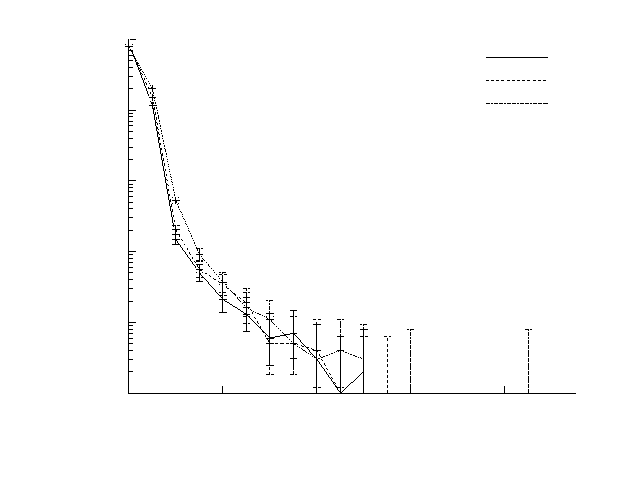
\includegraphics[width={288.00bp},height={216.00bp}]{images/r-simulations/electrons-general-view.eps}}%
    \gplfronttext
  \end{picture}%
\endgroup
}
%    \resizebox{!}{.33\textwidth}{% GNUPLOT: LaTeX picture with Postscript
\begingroup
  \makeatletter
  \providecommand\color[2][]{%
    \GenericError{(gnuplot) \space\space\space\@spaces}{%
      Package color not loaded in conjunction with
      terminal option `colourtext'%
    }{See the gnuplot documentation for explanation.%
    }{Either use 'blacktext' in gnuplot or load the package
      color.sty in LaTeX.}%
    \renewcommand\color[2][]{}%
  }%
  \providecommand\includegraphics[2][]{%
    \GenericError{(gnuplot) \space\space\space\@spaces}{%
      Package graphicx or graphics not loaded%
    }{See the gnuplot documentation for explanation.%
    }{The gnuplot epslatex terminal needs graphicx.sty or graphics.sty.}%
    \renewcommand\includegraphics[2][]{}%
  }%
  \providecommand\rotatebox[2]{#2}%
  \@ifundefined{ifGPcolor}{%
    \newif\ifGPcolor
    \GPcolorfalse
  }{}%
  \@ifundefined{ifGPblacktext}{%
    \newif\ifGPblacktext
    \GPblacktexttrue
  }{}%
  % define a \g@addto@macro without @ in the name:
  \let\gplgaddtomacro\g@addto@macro
  % define empty templates for all commands taking text:
  \gdef\gplbacktext{}%
  \gdef\gplfronttext{}%
  \makeatother
  \ifGPblacktext
    % no textcolor at all
    \def\colorrgb#1{}%
    \def\colorgray#1{}%
  \else
    % gray or color?
    \ifGPcolor
      \def\colorrgb#1{\color[rgb]{#1}}%
      \def\colorgray#1{\color[gray]{#1}}%
      \expandafter\def\csname LTw\endcsname{\color{white}}%
      \expandafter\def\csname LTb\endcsname{\color{black}}%
      \expandafter\def\csname LTa\endcsname{\color{black}}%
      \expandafter\def\csname LT0\endcsname{\color[rgb]{1,0,0}}%
      \expandafter\def\csname LT1\endcsname{\color[rgb]{0,1,0}}%
      \expandafter\def\csname LT2\endcsname{\color[rgb]{0,0,1}}%
      \expandafter\def\csname LT3\endcsname{\color[rgb]{1,0,1}}%
      \expandafter\def\csname LT4\endcsname{\color[rgb]{0,1,1}}%
      \expandafter\def\csname LT5\endcsname{\color[rgb]{1,1,0}}%
      \expandafter\def\csname LT6\endcsname{\color[rgb]{0,0,0}}%
      \expandafter\def\csname LT7\endcsname{\color[rgb]{1,0.3,0}}%
      \expandafter\def\csname LT8\endcsname{\color[rgb]{0.5,0.5,0.5}}%
    \else
      % gray
      \def\colorrgb#1{\color{black}}%
      \def\colorgray#1{\color[gray]{#1}}%
      \expandafter\def\csname LTw\endcsname{\color{white}}%
      \expandafter\def\csname LTb\endcsname{\color{black}}%
      \expandafter\def\csname LTa\endcsname{\color{black}}%
      \expandafter\def\csname LT0\endcsname{\color{black}}%
      \expandafter\def\csname LT1\endcsname{\color{black}}%
      \expandafter\def\csname LT2\endcsname{\color{black}}%
      \expandafter\def\csname LT3\endcsname{\color{black}}%
      \expandafter\def\csname LT4\endcsname{\color{black}}%
      \expandafter\def\csname LT5\endcsname{\color{black}}%
      \expandafter\def\csname LT6\endcsname{\color{black}}%
      \expandafter\def\csname LT7\endcsname{\color{black}}%
      \expandafter\def\csname LT8\endcsname{\color{black}}%
    \fi
  \fi
    \setlength{\unitlength}{0.0500bp}%
    \ifx\gptboxheight\undefined%
      \newlength{\gptboxheight}%
      \newlength{\gptboxwidth}%
      \newsavebox{\gptboxtext}%
    \fi%
    \setlength{\fboxrule}{0.5pt}%
    \setlength{\fboxsep}{1pt}%
    \definecolor{tbcol}{rgb}{1,1,1}%
\begin{picture}(5760.00,4320.00)%
    \gplgaddtomacro\gplbacktext{%
      \csname LTb\endcsname%%
      \put(946,4099){\makebox(0,0)[r]{\strut{}$1$}}%
      \put(946,704){\makebox(0,0)[r]{\strut{}$10^{-5}$}}%
      \put(946,1383){\makebox(0,0)[r]{\strut{}$10^{-4}$}}%
      \put(946,2062){\makebox(0,0)[r]{\strut{}$10^{-3}$}}%
      \put(946,2741){\makebox(0,0)[r]{\strut{}$10^{-2}$}}%
      \put(946,3420){\makebox(0,0)[r]{\strut{}$10^{-1}$}}%
      \put(1078,484){\makebox(0,0){\strut{}$0$}}%
      \put(1980,484){\makebox(0,0){\strut{}$0.1$}}%
      \put(2882,484){\makebox(0,0){\strut{}$0.2$}}%
      \put(3784,484){\makebox(0,0){\strut{}$0.3$}}%
      \put(4686,484){\makebox(0,0){\strut{}$0.4$}}%
    }%
    \gplgaddtomacro\gplfronttext{%
      \csname LTb\endcsname%%
      \put(4376,3926){\makebox(0,0)[r]{\strut{}$100~\text{ГэВ}$}}%
      \csname LTb\endcsname%%
      \put(4376,3706){\makebox(0,0)[r]{\strut{}$50~\text{ГэВ}$}}%
      \csname LTb\endcsname%%
      \put(4376,3486){\makebox(0,0)[r]{\strut{}$20~\text{ГэВ}$}}%
      \put(209,2401){\rotatebox{-270.00}{\makebox(0,0){\strut{}$p_{\pi^{-}}(E)$}}}%
      \put(3220,154){\makebox(0,0){\strut{}$R$}}%
    }%
    \gplbacktext
    \put(0,0){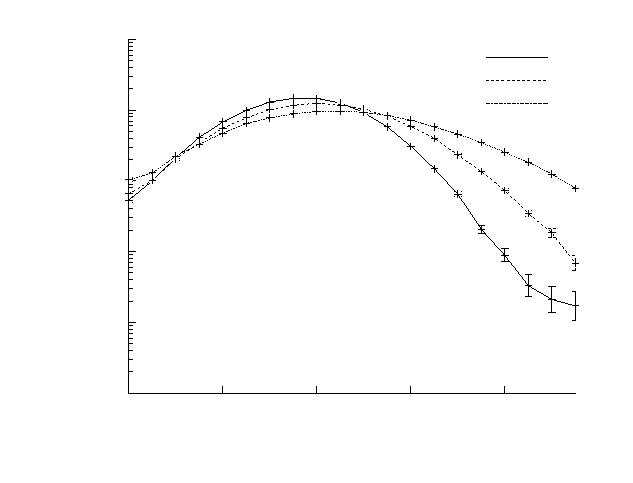
\includegraphics[width={288.00bp},height={216.00bp}]{images/r-simulations/pions-general-view.eps}}%
    \gplfronttext
  \end{picture}%
\endgroup
}
%    \caption{Результаты моделирования относительной доли энерговыделения
%    в периферийных ячейках HCAL
%    $R = (E_{HCAL} - E_{HCAL,C})/E_{HCAL}$
%    при различных энергиях $e^-$ и $\pi^-$}
%    \label{fig:r-distributions}
%\end{figure}
\begin{figure}[ht]
    \centering
    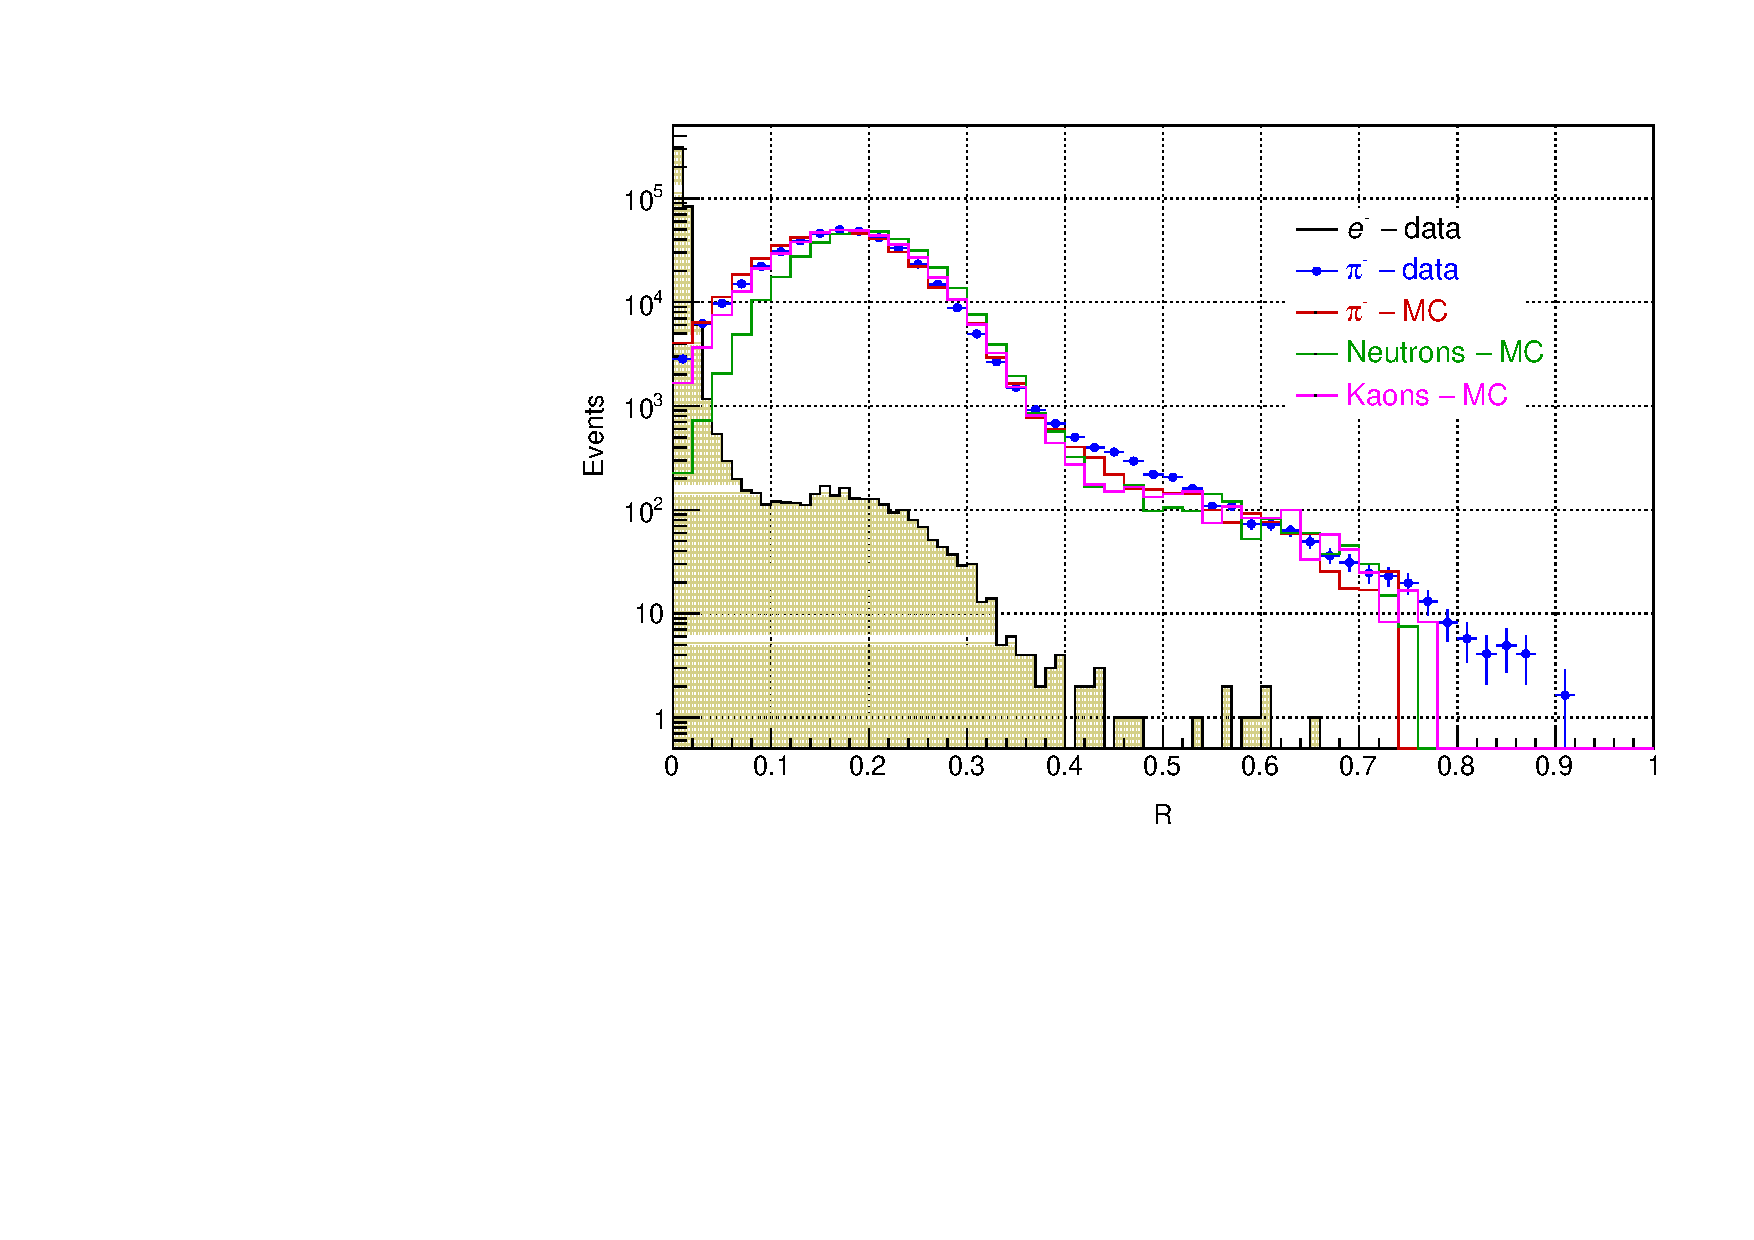
\includegraphics[width=.75\textwidth]{images/r-simulations/HCraio-e-428-pi-3924-MC.pdf}
    \caption{Распределения $R$ для различных типов частиц совместно с
    данными полученными на калибровочных пучках}
    \label{fig:r-dist-realdata}
\end{figure}

В результате перенормировки на реальные данные, рабоча точка была
скорректирована в сторону более консервативной оценки, и при анализе
данных использовалось значение $R_{th} = 0{,}06$.

\subsection{Фоновые процессы}

В видимой постановке модуль HCAL0 играет роль ветирующего
калориметра с длиной адронного взаимодействия $\simeq 7{,}43~ \lambda_I$,
эффективность которого можно определить как обратную вероятность
адрону преодолеть модуль без ядерного взаимодействия.
Для нейтронов эта вероятность
составляет~$P_{n,PT} = e^{-7{,}43}\simeq5{,}9\times 10^{-4}$.

Грубые консервативные оценки можно сделать
согласно сечениям из работы~\cite{leading-neutron-hera}, утверждая что доля
событий в которых образовался нейтральный адрон (нейтрон или $\bar{K}_{0}$)
с энергией больше $1~\text{ГэВ}$ не превышает $f \simeq 5\%$.
Тогда общая вероятность зарегистрировать нейтральный адрон
в HCAL2,3 с $R < 0{,}06$, который образовался в ECAL, прошёл без
взаимодействия HCAL0 не превышает $\simeq 2.7\cdot 10^{-8}$.
%$0{,}05 \times 5{,}9 \cdot 10^{-4} \times 2{,}8\cdot 10^{-2} \simeq 2.7\cdot 10^{-8}$.

Более точная консервативная оценка полученная при
помощи \acrshort{mc}-моделирования, скорректированная на
распады учитывающая измеренный экспериментально выход нейтральных
адронов составляет $0{,}02 \pm 0{,}08$ для
нейтронов и $0{,}14\pm0{,}045$ для $K^0$.

В интегральную оценку фона $0{,}17\pm0{,}046$ также был включён
вклад от адронного загрязнения пучка, с учётом эффективности
SRD и системы мечения и ошибки идентификации мюонных пар.

\begin{comment}
с вероятностью на уровне $10^{-4}$ событий ожидается
адронное загрязнения пучка -- избежавшие регистрации
SRD $\pi^{-}$ и $K^{-}$-мезоны
могут распадаться с образованием нейтрино
и электронов в процессах $K^{-} \rightarrow \pi^{0} e^{-} \nu$, $\pi^{-} \rightarrow e^{-} \nu$.
Эта адронная компонента, а так же мюоны и гамма-кванты высоких
энергий способны проходить толстые поглотители
с низким энерговыделением (англ. \emph{punch-through})~\cite{punch-trough-photons}.

Оценка вклада фоновых процессов вследствие адронизации компоненты
электромагнитного ливня, а также эффектов punch-through выполнялась
посредством моделирования Монте-Карло.  % и была верифицирована ?

%\subsection{Оценка фонового вклада отрицательных пионов}

Распределения относительной доли в периферийных ячейках $R$ для $e^{-}$
и $\pi^{-}$ и различных энергий приведены на рисунке \ref{fig:r-distributions},
откуда видно, что $R$ для обоих типов событий слабо зависит
от энергии, и определяется в основном ливня.

Оценка частиц проходящих VETO и HCAL0 без взаимодействия вычислялась
посредством Монте-Карло моделирования с перенормировкой.
Итоговые относительные оценки фона от различных источников
приведены в таблице~\ref{tab:alps-background}.

\begin{table}[]
    \centering
    \begin{tabular}{rl}
         Источник фона & Относительный вклад  \\ \hline
         $n$    & $(7{,}04 \pm 2.82)\cdot10^{-14}$  \\
         $K^0$  & $(4{,}93\pm1{,}6)\cdot10^{-13}$  \\
         Пучковые $\pi^{-}$, $K\rightarrow \pi^{-} + X$ & $(2{,}11\pm0{,}7) \cdot 10^{-14}$ \\
         $2\mu$ & $< 3 \cdot 10^{-15}$ \\ \hline
         Всего & $(6\pm1{,}6)\cdot10^{-13}$
    \end{tabular}
    \caption{Основные источники фона}
    \label{tab:alps-background}
\end{table}

\end{comment}

%Интегральная оценка вклада пучковых $\pi^-$ (в том числе
%в результате процессов $K \rightarrow \pi^{-} + X$) даёт
%консервативную оценку в $(2{,}11 \pm 0{,}69)\cdot 10^{-14}$
%событий для $R \le 0{,}6$.

%Для $E_0 = 100~\text{ГэВ}$ порог составлял $E_{th} = 85~\text{ГэВ}$ для
%видимой сигнатуры и $50~\text{ГэВ}$ для невидимой. В видимой
%моде ветирование осуществлялось только первым модулем HCAL.

\subsection{Вычисление исключённой области}

На основании результатов моделирования для анализа энергетический
верхний порог для ECAL в видимой моде выбран равным $85~\text{ГэВ}$,
%(соответствующий триггеру)
для невидимой моды порог был установлен в $50~\text{ГэВ}$, для VETO
и HCAL0 энерговыделение не должно было превосходить $E_{MIP}/2$.

\begin{comment}
\begin{figure}
    \centering
    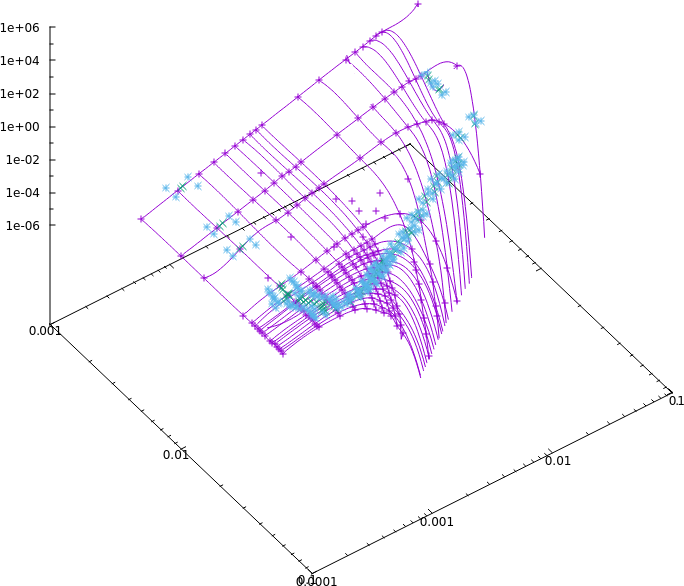
\includegraphics[width=0.33\linewidth]{images//illustrative/alps-analysis.png}
    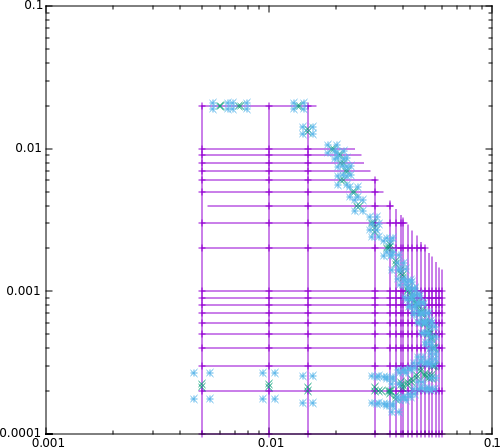
\includegraphics[width=0.33\linewidth]{images//illustrative/alp-analysis-top-view.png}
    \caption{Иллюстрация работы дихотомического алгоритма для отыскания
    области принятия гипотезы $H_0$}
    \label{fig:alps-dichotomy-search}
\end{figure}
\end{comment}

\begin{figure}[ht]
    \centering
    \resizebox{!}{.36\textwidth}{% GNUPLOT: LaTeX picture with Postscript
\begingroup
  \makeatletter
  \providecommand\color[2][]{%
    \GenericError{(gnuplot) \space\space\space\@spaces}{%
      Package color not loaded in conjunction with
      terminal option `colourtext'%
    }{See the gnuplot documentation for explanation.%
    }{Either use 'blacktext' in gnuplot or load the package
      color.sty in LaTeX.}%
    \renewcommand\color[2][]{}%
  }%
  \providecommand\includegraphics[2][]{%
    \GenericError{(gnuplot) \space\space\space\@spaces}{%
      Package graphicx or graphics not loaded%
    }{See the gnuplot documentation for explanation.%
    }{The gnuplot epslatex terminal needs graphicx.sty or graphics.sty.}%
    \renewcommand\includegraphics[2][]{}%
  }%
  \providecommand\rotatebox[2]{#2}%
  \@ifundefined{ifGPcolor}{%
    \newif\ifGPcolor
    \GPcolortrue
  }{}%
  \@ifundefined{ifGPblacktext}{%
    \newif\ifGPblacktext
    \GPblacktexttrue
  }{}%
  % define a \g@addto@macro without @ in the name:
  \let\gplgaddtomacro\g@addto@macro
  % define empty templates for all commands taking text:
  \gdef\gplbacktext{}%
  \gdef\gplfronttext{}%
  \makeatother
  \ifGPblacktext
    % no textcolor at all
    \def\colorrgb#1{}%
    \def\colorgray#1{}%
  \else
    % gray or color?
    \ifGPcolor
      \def\colorrgb#1{\color[rgb]{#1}}%
      \def\colorgray#1{\color[gray]{#1}}%
      \expandafter\def\csname LTw\endcsname{\color{white}}%
      \expandafter\def\csname LTb\endcsname{\color{black}}%
      \expandafter\def\csname LTa\endcsname{\color{black}}%
      \expandafter\def\csname LT0\endcsname{\color[rgb]{1,0,0}}%
      \expandafter\def\csname LT1\endcsname{\color[rgb]{0,1,0}}%
      \expandafter\def\csname LT2\endcsname{\color[rgb]{0,0,1}}%
      \expandafter\def\csname LT3\endcsname{\color[rgb]{1,0,1}}%
      \expandafter\def\csname LT4\endcsname{\color[rgb]{0,1,1}}%
      \expandafter\def\csname LT5\endcsname{\color[rgb]{1,1,0}}%
      \expandafter\def\csname LT6\endcsname{\color[rgb]{0,0,0}}%
      \expandafter\def\csname LT7\endcsname{\color[rgb]{1,0.3,0}}%
      \expandafter\def\csname LT8\endcsname{\color[rgb]{0.5,0.5,0.5}}%
    \else
      % gray
      \def\colorrgb#1{\color{black}}%
      \def\colorgray#1{\color[gray]{#1}}%
      \expandafter\def\csname LTw\endcsname{\color{white}}%
      \expandafter\def\csname LTb\endcsname{\color{black}}%
      \expandafter\def\csname LTa\endcsname{\color{black}}%
      \expandafter\def\csname LT0\endcsname{\color{black}}%
      \expandafter\def\csname LT1\endcsname{\color{black}}%
      \expandafter\def\csname LT2\endcsname{\color{black}}%
      \expandafter\def\csname LT3\endcsname{\color{black}}%
      \expandafter\def\csname LT4\endcsname{\color{black}}%
      \expandafter\def\csname LT5\endcsname{\color{black}}%
      \expandafter\def\csname LT6\endcsname{\color{black}}%
      \expandafter\def\csname LT7\endcsname{\color{black}}%
      \expandafter\def\csname LT8\endcsname{\color{black}}%
    \fi
  \fi
    \setlength{\unitlength}{0.0500bp}%
    \ifx\gptboxheight\undefined%
      \newlength{\gptboxheight}%
      \newlength{\gptboxwidth}%
      \newsavebox{\gptboxtext}%
    \fi%
    \setlength{\fboxrule}{0.5pt}%
    \setlength{\fboxsep}{1pt}%
    \definecolor{tbcol}{rgb}{1,1,1}%
\begin{picture}(5668.00,3684.00)%
    \gplgaddtomacro\gplbacktext{%
      \csname LTb\endcsname%%
      \put(1045,843){\makebox(0,0)[r]{\strut{}$10^{-2}$}}%
      \put(3012,78){\makebox(0,0)[l]{\strut{}$10^{-4}$}}%
      \put(4316,697){\makebox(0,0)[l]{\strut{}$10^{-3}$}}%
      \put(5620,1316){\makebox(0,0)[l]{\strut{}$10^{-2}$}}%
      \put(101,1861){\makebox(0,0)[r]{\strut{}$10^{-1}$}}%
      \put(101,2130){\makebox(0,0)[r]{\strut{}$10^{1}$}}%
      \put(101,2399){\makebox(0,0)[r]{\strut{}$10^{3}$}}%
      \put(101,2669){\makebox(0,0)[r]{\strut{}$10^{5}$}}%
    }%
    \gplgaddtomacro\gplfronttext{%
      \csname LTb\endcsname%%
      \put(748,467){\makebox(0,0){\strut{}$m_a$, ГэВ}}%
      \put(4920,467){\makebox(0,0){\strut{}$\epsilon_{a \gamma \gamma}$}}%
      \put(-781,2265){\makebox(0,0){\strut{}N}}%
    }%
    \gplbacktext
    \put(8bp,10bp){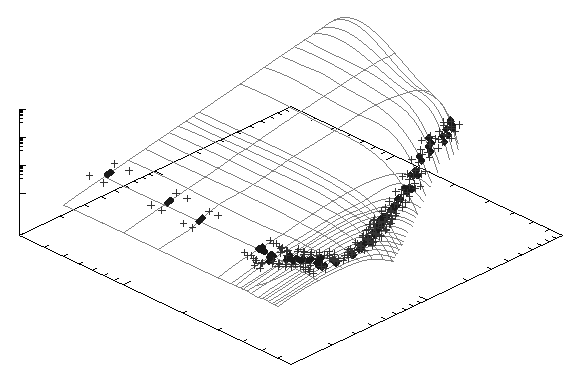
\includegraphics[width={268.40bp},height={184.20bp}]{images/alps-search/surf-1.eps}}%
    \gplfronttext
  \end{picture}%
\endgroup
}
    \caption{Иллюстрация работы дихотомического алгоритма для отыскания
    исключённой области ALP}
    \label{fig:alps-dichotomy-search-isometric}
\end{figure}

\begin{comment}
В \textbf{разделе 4.2} дано описание процедуры
реконструкции и анализа ALP в постановках на $e^{-}$ пучке
$100 \text{ГэВ}$ для невидимой % signature 2
$e^- + Z\rightarrow e^- + Z +a$ и видимой  
($a \rightarrow \gamma\gamma$) сигнатур % signature 1
на данных 2016-2018г. Приводятся численные оценки доказывающие
соответствие ширины $\Gamma_a = g^2_{a \gamma \gamma} m^3_a / 64 \pi$,
распадной базе NA64. Показано, что на установке NA64 среди параметров
для выделения сигнальных событий, основными являются:
\begin{itemize}
    \item Верхний порог депонированной энергии в электромагнитном
    калориметре $E_{ECAL} \lesssim 85 ~\text{ГэВ}$ для видимой моды
    и $E_{ECAL} \lesssim 50 ~\text{ГэВ}$ для невидимой моды.
    \item Ограничение на отношение ливневой энергии в периферийных
    ячейках модуля адронного калориметра $E^P_{HCAL}$ к полной $E_{HCAL}$:
    $R = E^{P}_{HCAL}/E_{HCAL}$, полученное на основе
    моделирования Монте-Карло с применением генераторов описанных в
    предыдущих разделах.
    \item Порог на энергию синхротронного излучения в системе мечения,
    для идентификации $e^-$.
    \item Порог на ветирющий детектор (\texttt{VETO}) для невидимой
    моды.
\end{itemize}
Также в разделе приводятся оценки фона для
статистики~$2{,}84 \times 10^{11}$ электронных событий.

В \textbf{разделе 4.3} приводятся результаты моделирования
$R$-фактора. Помимо результатов опубликованных
в статьях \cite{alps-PRL, alps-PRD}, приводятся также результаты
моделирования для других номинальных энергий
инициирующего~$e^{-}$,~см.~рис.~\eqref{fig:R-dist}.
\begin{figure}[ht]
    \begin{subfigure}{0.49\textwidth}
        \includegraphics[width=0.95\linewidth]{img/r-dist-pi-.png}
        \label{fig:r-dist-hadrons}
    \end{subfigure}
    \begin{subfigure}{0.49\textwidth}
        \includegraphics[width=0.95\linewidth]{img/r-dist-e-.png}
        \label{fig:r-dist-leptons}
    \end{subfigure}
    %\includegraphics[width=0.75\linewidth]{img/R-dist-PRL.png}
    \caption{Сравнение распределений параметра $R$ для адронного и электронного пучков
    различных энергий.}
    \label{fig:R-dist}
\end{figure}
%В разделе приведены оценки фонов. %, в частности показано, что основной вклад в фон вносит
%механизм (2), особенно распады $K^0_{S,L}$ на лету.

В \textbf{разделе 4.4} приведены результаты обработки, см. рис \ref{fig:biplot-prl}.

На ...-а показана выборка $3 \times 10^4$ событий от
реакции $e^-+Z$ полученных из начальной статистики при условии
наличия в пучке электрона.  %, идентифицированного по сигнатуре в SRD.
Наглядной особенностью данного графика являются события из
горизонтальной полосы с $E_\text{HCAL} \approx 10~\text{ГэВ}$ обусловлены
димюонным рождением. Эти события использовались для количественной верификации
чувствительности установке в интервале энергий $1-100~\text{ГэВ}$.

Ветирование электромагнитного калориметра толстым сцинтилляционным детектором
оставляет примерно $7 \times 10^3$ событий, показанных на ...-б. Эти события
соответствуют нейтральным адронам, депонирующим остаток энергии после в модулях
\texttt{HCAL1-3}. Сохранение полной энергии соответствует распределению
этих событий вдоль диагонали~$E_\texttt{ECAL} + E_\texttt{HCAL} \approx 100~\text{ГэВ}$.

Сигнальные события видимой моды должны проявляться в виде избытка событий $(E_\text{ECAL}, E_\text{HCAL})$ внутри сигнального окна 1 (диагональный полигон на ...-в), с
учётом разрешения детектора и ограничению $R < 0{,}06$. Сигнальное окно 2,
определяемое как $0 \lesssim E_\text{ECAL} \lesssim 55~\text{ГэВ}$,
$E_\text{HCAL} \lesssim 1~\text{ГэВ}$, соответствует событиям с большой потерей
энергии/.

%Были рассмотрены следующие фоны, имитирующие распад $a \rightarrow \gamma\gamma$ в HCAL2,3:
%\begin{enumerate}
%    \item Рождение ведущего нейтрона ($n$) или $K^0$ в ECAL: $e^- A \rightarrow n(K^0) + m\pi^0 + X$.
%    \item Сопутствующие $\pi^0$ распадаются в ECAL; малая активность в VETO и HCAL1.
%    \item $\pi^-$ и $K^-$ в пучке, не отфильтрованные SRD, с последующим распадом или тормозным излучением.
%    \item Мюоны от димюонных пар, порождённых в ECAL.
%\end{enumerate}

\begin{figure}
    \centering
    \includegraphics[width=1\linewidth]{img/alps-prl-biplot.png}
    \caption{}
    \label{fig:biplot-prl}
\end{figure}

В \textbf{разделе 4.5} дано описание алгоритма дихотомического
поиска кривой исключения для порога
статистической значимости $\alpha = 0{,}1$ на статистике
соответствующей~$2{,}84 \times 10^{11}$ электронных событий
набранной~NA64 в указанной постановке (рис. \ref{fig:PRL-excPlots-pub}).

%(самоцитирование по статье \cite{mine-alps-PRL}
\begin{figure}
    \centering
    \label{fig:PRL-excPlots}
    %\includegraphics[width=0.5\linewidth]{img/alps-self-quotation.png}  % PRD
    % ^^^ https://cds.cern.ch/record/2741614/plots)
    \begin{subfigure}{0.49\textwidth}
        \includegraphics[width=.99\textwidth]{img/alps-search-1.png}
        \caption{Дихотомический поиск кривой чувствительности в
        параметрическом пространстве для $\alpha = 0{,}9$.}
        \label{fig:PRL-excPlots-raw}
    \end{subfigure}
    \begin{subfigure}{0.49\textwidth}
        \includegraphics[width=.99\linewidth]{img/ALPs-excl-plot-PRL.png}
        \caption{Сравнительная визуализация в
        параметрическом пространстве масс (псевдо-)скаляров $m_a$ против
        константы смешивания $g_{a \gamma \gamma}$}
        \label{fig:PRL-excPlots-pub}
    \end{subfigure}
    \caption{Работа алгоритма дихотомического поиска для уровня статистической
    значимости $\alpha = 0{,}1$ (слева) и  (справа) с указанием
    ограничений экспериментов BABAR, E137, E141, LEP, PrimEX,
    CHARM, NuCAL, актуальных на момент публикации \cite{alps-PRL}. Жёлтым выделены
    ограничения соответствующих теоретических моделей.}
\end{figure}
\end{comment}
